\RequirePackage{lineno} 
\documentclass[a4paper,11pt,spanish]{article}

\usepackage[spanish]{babel}
\usepackage[utf8]{inputenc}
\usepackage{url}
\usepackage{graphicx} 
\usepackage{slashbox}
\usepackage{longtable}
\usepackage{multirow}
\usepackage{colortbl}
\usepackage{color}
\usepackage{subfloat}
\usepackage{lineno}
\usepackage{tikz}
\usepackage{fancybox}
%\usepackage{hyperref}
\usepackage{bigfoot} %for split long footnotes
\usepackage{textcomp}
\usepackage{amsmath}
\usepackage{babel}
\usepackage{listings} %for c++ code
\definecolor{dkgreen}{rgb}{0,0.6,0}
\definecolor{gray}{rgb}{0.5,0.5,0.5}
\definecolor{mauve}{rgb}{0.58,0,0.82}
\usepackage{makeidx}
\lstset{ %
  language=C++,                % the language of the code
  basicstyle=\footnotesize,           % the size of the fonts that are used for the code
  %numbers=left,                   % where to put the line-numbers
  %numberstyle=\tiny\color{gray},  % the style that is used for the line-numbers
  %stepnumber=2,                   % the step between two line-numbers. If it's 1, each line  will be numbered
  %numbersep=5pt,                  % how far the line-numbers are from the code
  backgroundcolor=\color{white},      % choose the background color. You must add \usepackage{color}
  showspaces=false,               % show spaces adding particular underscores
  showstringspaces=false,         % underline spaces within strings
  showtabs=false,                 % show tabs within strings adding particular underscores
  frame=single,                   % adds a frame around the code
  rulecolor=\color{black},        % if not set, the frame-color may be changed on line-breaks within not-black text (e.g. commens (green here))
  tabsize=8,                      % sets default tabsize to 2 spaces
  captionpos=b,                   % sets the caption-position to bottom
  breaklines=false,                % sets automatic line breaking
  breakatwhitespace=true,        % sets if automatic breaks should only happen at whitespace
  title=\lstname,                   % show the filename of files included with \lstinputlisting;
  basicstyle=\scriptsize,                             % also try caption instead of title
  keywordstyle=\color{blue},          % keyword style
  commentstyle=\color{dkgreen},       % comment style
  stringstyle=\color{mauve},         % string literal style
  %escapeinside={\%*}{*)},            % if you want to add a comment within your code
  %morekeywords={*,...}               % if you want to add more keywords to the set
}

\usepackage{subfig}

\makeindex


% \usepackage{gantt}
% \setlength{\textheight}{24cm}
% \textwidth=16.5cm
% \topmargin=0cm
% \oddsidemargin=0cm
% \parindent=10mm
% \definecolor{shadecolor}{rgb}{1, 0, 0}
\begin{document}
%\linenumbers %activar nro de lineas
\pagestyle{empty}
\begin{center}

	\bigskip
	\bigskip
	
%	{\bf\Large Algoritmo para la detección de objetos planos aplicado a videos en un ambiente controlado.} \\
	{\bf\Large Método para detección y seguimiento de objetos con aplicaciones en Realidad Aumentada} \\
%	{\bf\Large Algoritmo para la detección de objetos planos en videos en un ambiente controlado.} \\

	\bigskip
	\bigskip

	\large Christian Nicolás Pfarher\\


  	\bigskip
  	\bigskip
	
	Punto de control N$^{\circ}$ 4: \\	
		\begin{description}
			\item Pre-procesamiento para lograr posibles mejoras de velocidad, en tiempo de ejecución
			\item Análisis homográfico, proyecciones y transformaciones
			\item Superposición de contenido sobre el objeto detectado
		\end{description}

	 
	\bigskip
	
	Director\\
	\textit{Dr. Enrique Marcelo Albornoz}\\
	\bigskip
	Codirector\\
	\textit{Dr. César Martínez}\\
	
	\bigskip
	\bigskip
	\bigskip
	\bigskip
	\bigskip
	\bigskip
	\textit{\today}\\
	

	\vfill
	\begin{figure}[tbhp]
		\centerline{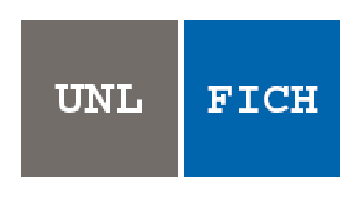
\includegraphics[scale=0.6]{img/fich_unl}}
	\end{figure}
	
  	{Ingeniería Informática}\\
  	{Facultad de Ingeniería y Ciencias Hídricas}\\
    {UNIVERSIDAD NACIONAL DEL LITORAL}	
\end{center}

\bigskip
\bigskip

\newpage
\tableofcontents
%\printindex
\newpage

\pagestyle{plain}

\section{Pre-procesamiento para lograr posibles mejoras de velocidad, en tiempo de ejecución}
En esta sección, se plantearán algunas herramientas como posibles alternativas a aplicar con el objetivo de lograr mejoras de velocidad en tiempo de ejecución.

% Transformación de imágenes con operaciones morfológicas:
% Los filtros morfológicos, definen operaciones que transforman imágenes mediante la aplicación de elementos con formas predefinidas. La forma en que estos elementos intersectan la vecinidad de un pixel, determina el resultado de la operación.
Como es sabido, tanto el uso del método SURF para la extracción de características como la búsqueda de coincidencias entre imágenes, conllevan un gran tiempo de procesamiento, el cual se convierte en un factor clave a la hora de lograr mayor fluidez en la reproducción del flujo de video \cite{citeulike:9456628, Beis:1997:SIU:794189.794431, Friedman:1977:AFB:355744.355745, Liu04aninvestigation}. Para reducir este problema, se recurre a técnicas para detectar la parte cambiante de la imagen, de tal forma de aplicar el procesamiento solo en una región de la imagen capturada en vez de en su totalidad de forma de reducir los datos a procesar. Para ello, se utilizan diferentes herramientas de procesamiento de imágenes en el siguiente orden: conversión a escala de grises, diferencia de imágenes, umbral, erosión, dilatación y bounding box. Estas herramientas, fueron elegidas debido a su grado de simpleza y bajo tiempo de procesamiento que requieren para llevarse a cabo, de forma tal de influenciar en la menor medida posible el tiempo de proceso total del algoritmo.

\subsection{Conversión a escala de grises}
La conversión a escala de grises, consiste en convertir la imagen de un espacio de color a otro, en este caso se convierte del espacio de colores RGB o BGR a escala de grises. Para el cálculo del valor de gris se usa la fórmula perceptualmente ponderada $Y=(0.299)R+(0.587)G+0.114B$ donde $R$, $G$ y $B$ representan los canales rojo, verde y azul de la imagen respectivamente.

Este proceso es llevado a cabo mediante la función provista por la librería OpenCV $cvCvtColor(const CvArr* src, CvArr* dst, int code)$ con el parámetro $code=CV\_RGB2GRAY$.

% Cabe aclarar, que se optó por trabajar con escalas de grises ya que esto implica menores tiempos de cálculos en los procesos y el método de extracción de características trabaja solo con imágenes de estas cualidades. 

\subsection{Diferencia de imágenes}
La diferencia de imágenes se aplica con el objetivo de lograr distinguir el cambio en la imagen cuadro a cuadro. Consiste en calcular el valor absoluto de la diferencia entre el cuadro $F$ del flujo de video capturado en el tiempo $t$ (actual) y el capturado en $t-1$ (anterior), es decir: $D=|F_{t}-F{_{t-1}}|$ (pixel a pixel). El resultado de la operación, es una imagen $D$ en la que se observa la parte que ha cambiado de una imagen a otra.

\subsection{Threshold}
\label{subsub_ymbral}
A partir de la imagen diferencia $D$ obtenida anteriormente, se procede con la aplicación de un umbral binario de la forma \eqref{equation_umbral_binario} para remover ruido. Se asigna el valor $valorMaximo=255$ a los píxeles que superen el umbral con un valor definido empíricamente ($u=50$) y $0$ a los demás píxeles, obteniéndose como resultado una nueva imagen $I$.

\begin{equation}
\label{equation_umbral_binario}
I= 
\begin{cases} x & \text{si $valorMaximo>u$,}
\\
0 &\text{en otro caso}
\end{cases}
\end{equation}

%cvThreshold (50, 255, CV\_THRESH\_BINARY) y agregar grafico del umbral
\subsection{Erosión y dilatación}
Las erosión y dilatación son dos de las principales operaciones morfológicas usadas en variedad de contextos como remoción de ruido, aislación/unión de elementos, etc.

En este contexto, estas operaciones serán aplicadas para eliminar puntos aislados o ruido que no haya sido removido mediante el umbral descripto anteriormente en \ref{subsub_ymbral}, de forma que el Bounding Box sea detectado correctamente en una próxima etapa.

Tanto la \textbf{Dilatación} como la \textbf{Erosión} consisten en la convolución de una imagen (o una parte de ella) con un kernel que puede ser de diferentes formas o tamaños y que posee un ``punto de anclaje'' también llamado punto central del kernel.
% Estos dos filtros operan sobre un conjunto de píxeles vecinos alrededor de cada píxel de la imagen sobre la cual es aplicada la operación.

La \emph{erosión}, reemplaza al píxel actual con el valor mínimo de la vecindad definida, mientras que la \emph{dilatación} es la operación complementaria a la anterior, es decir, que reemplaza el píxel actual con el valor máximo del conjunto de píxeles vecinos. Así, en el caso de una imagen binaria (sólo contiene píxeles negros (0) y blancos (255)), cada píxel es reemplazado por uno negro o blanco. En una imagen erosionada, el tamaño de los objetos se ve reducido y el ruido es eliminado. En el caso de la dilatación, los objetos crecen en su tamaño y algunos de los espacios dentro de ellos son rellenados.
% Una buena forma de ver el efecto de este operador es en términos de una imagen con fondo negro y objetos blancos. Cuando se aplica la erosión, si un píxel del filtro aplicado esta sobre el fondo, luego el pixel sobre el cuál se esta aplicando la erosión resultará con el valor del fondo. Mientras, que en el caso de la dilatación, si el filtro toca un objeto sobre el fodno, el pixel será asignado al valor del blanco. 
% poner que máscara se usa y poner imagen
% cvErode(frameDiferencia, frameDiferencia, NULL, 2);
% cvDilate(frameDiferencia, frameDiferencia, NULL, 2);
%http://opencv.willowgarage.com/documentation/miscellaneous_image_transformations.html?highlight=cvthreshold#cvThreshold

\subsection{Bounding Box}
Luego del procesamiento anterior, es el momento de detectar el rectángulo más pequeño que encierra completamente todos los puntos cuyo valor de píxel no es completamente 0, es decir, píxeles no negros. A esto se le llama Bounding Box y puede ser utilizado para descartar regiones de la imagen que no necesitamos procesar en un algoritmo. Debido que anteriormente hemos eliminado el ruido mediante las operaciones de umbral, dilatación y erosión, nos aseguramos de esta forma el poder encontrar un único Bounding Box válido. Este contedrá la parte cambiante de la imagen sobre la que detectaremos características y haremos el posterior proceso de correspondencia y detección de la ubicación del objetivo a detectar.
% boundingRect \= cvBoundingRect(frameDiferencia, 0);
% areabounding mayor que threshold

\section{Análisis homográfico, proyecciones y transformaciones}
Hasta el momento, se han mencionado diversas técnicas que se aplican a la imagen para detectar características distinguibles de las mismas (puntos claves y vectores descriptores), de forma de poder identificarla en un contexto específico. A continuación se expondrá la forma por la cual se detecta si el objeto a detectar está presente en el flujo de video capturado, además de identificar su posición respecto a la cámara. Para ello, es necesario introducir algunos conceptos básicos de formación de la imagen que se explicarán a continuación.
% Para ello, se tratarán diversos temas entre los que podemos mencionar: el proceso de formación de la imagen y el modelo de cámara oscura, la calibración de la cámara y los parámetros extrínsecos e intrínsecos de la misma, 
\subsection{Introducción}
El principal componente para la visión en una escena es la luz. La misma proviene como un rayo que sale de una fuente (por ejemplo: el sol o una lámpara) y viaja a través del espacio hasta intersectar un objeto. Aquí, parte de la luz es absorbida y otra reflejada (percibida como el color) la cual es captada por los ojos (o cámara) y recogida en la retina (o imagen).
% La geometría de esta estructura, es de particular importancia práctica en visión computacional.

Existen diversos dispositivos para obtener imágenes, uno de los más comunes, es la cámara digital. Ésta captura la escena mediante la proyección de luz en un sensor a través del lente de la cámara. El hecho de que la imagen se forma a través de la proyección de la escena 3D en un plano 2D, implica la existencia de importantes relaciones entre la escena y su imagen, y es la geometría proyectiva la herramienta usada para describir y caracterizar en términos matemáticos este proceso de formación de la imagen \cite{citeulike:3484001, citeulike:9456628}.

Para entender un poco más el proceso, existe un modelo teórico útil denominado \textbf{modelo de caja oscura}, del inglés: \textbf{``pinhole camera model''} \cite{bb38231, citeulike:3484001} con el cual se puede entender la geometría básica en la proyección de rayos y que será expuesto en \ref{subsubsection_formacion_imagen}. Sin embargo, un modelo de este tipo no puede ser aplicado realmente para obtener imágenes en la vida real, ya que el mismo no puede recoger la suficiente cantidad de luz en una exposición rápida. Es por esto que las cámaras usan lentes (los cuales introducen distorsiones no deseables) para obtener más luz de la disponible para un punto dado.
% Un ``pinhole''  un orificio de apertura pequeña en el centro de una pared imaginaria. 
Estas desviaciones provocadas por la lente, pueden ser corregidas matemáticamente a través de la calibración de la cámara, técnica mediante la cual se puede obtener tanto el modelo geométrico de la cámara como el modelo de distorsión de la lente, los cuales pasan a formar parte de los parámetros intrínsecos.

\subsection{Formación de la imagen}
\label{subsubsection_formacion_imagen}
El proceso de formación de la imagen no ha cambiado desde los comienzos de la fotografía \cite{citeulike:9456628}. La luz proveniente de la escena observada, es capturada por la cámara a través de la apertura frontal y los rayos de luz impactan en el plano de la imagen (o sensor de imagen) localizado por detrás de la cámara, en donde un lente es usado para concentrar los rayos provenientes de los diferentes elementos de la escena. Este proceso, se ilustra en la Fig. \ref{figura_image_formation_1}, donde $do$ es la distancia de la lente al objeto observado, $di$ es la distancia de la lente al plano de la imagen y $f$ es denominada \textbf{distancia focal}. Estas variables, se encuentran relacionadas mediante la ecuación de la lente \eqref{eq_ecuacion_lente}.

\begin{figure}[tbhp]
\centerline{\includegraphics[scale=0.5]{entregable04/img/imgformation1}}
\caption{Formación de la imagen. Adaptada de \cite{citeulike:9456628}. }
\label{figura_image_formation_1}
\end{figure}

\begin{equation}
 \frac{1}{f}=\frac{1}{do}+\frac{1}{di}
\label{eq_ecuacion_lente}
\end{equation}

En visión computacional, este modelo de cámara puede ser simplificado mediante ciertas consideraciones:
\begin{itemize}
 \item Se asume nulo el efecto de la lente (distorsión),
 \item Se considera una cámara con una apertura infinitesimal: de esta forma sólo se considera el rayo central,
 \item Se asume $do>>di$: esto significa que el plano de la imagen está en la posición de la distancia focal (enfocado),
 \item De la geometría del sistema, puede observarse que el objeto resulta invertido en el plano de la imagen: se puede obtener una imagen idéntica pero no invertida, simplemente posicionando el plano de la imagen en frente de la lente (aunque esto no es físicamente posible, es completamente equivalente desde un punto de vista matemático).
\end{itemize}
Este modelo simplificado, es conocido como ``modelo de cámara oscura'' y se representa en la Fig. \ref{figura_image_formation_2}
\begin{figure}[tbhp]
\centerline{\includegraphics[scale=0.5]{entregable04/img/imgformation2}}
\caption{Modelo pin\-hole de la cámara. Adaptada de \cite{citeulike:9456628}.}
\label{figura_image_formation_2}
\end{figure}

Usando la ley de similitud de triángulos y observando el modelo mencionado, se puede derivar la ecuación de proyección \eqref{eq_ecuacion_proy} de la cual se desprende que: el tamaño $hi$ de un objeto de altura $ho$ en el plano imagen, resulta inversamente proporcional a la distancia $do$ entre la cámara y el objeto. Esta relación, es fácilmente observable: cuando se fotografía un objeto cercano a la cámara, el mismo  aparece de mayor tamaño en el plano de la imagen; por el contrario si el objeto es alejado de la misma, éste aparece de menores dimensiones en el plano de la imagen. De esta manera se puede obtener la posición de un punto 3D de la escena, en el plano imagen.

\begin{equation}
 hi=f\frac{ho}{do}
\label{eq_ecuacion_proy}
\end{equation}

\subsection{Calibración de la cámara}
De la sección \ref{subsubsection_formacion_imagen}, se vio que los parámetros esenciales de la cámara son la distancia focal y el tamaño del plano de la imagen.
% (que define el campo de vista de la cámara). 
Cuando se trata de imágenes digitales, la cantidad de píxeles en el plano de la imagen resulta ser otro parámetro importante a determinar con el objetivo de calcular la posición %en coordenadas 
de un punto de la escena en el plano de la imagen. Si consideramos la línea ortogonal al plano de la imagen proveniente del punto focal, necesitamos saber en que píxel esta línea perfora el plano de la imagen. Este punto es llamado \textbf{``punto principal''}. Si bien resulta lógico asumir que este punto está en el centro del plano de la imagen, esto sólo se puede aseverar en condiciones ideales, ya que en la práctica el mismo se encuentra desplazado dependiendo de la precisión de fabricación de la cámara. Es por ello que se necesita un proceso de calibración de la misma.

La calibración de la cámara es el proceso, por el cual son obtenidos diferentes parámetros tales como la matriz de esta y los parámetros de distorsión (ignorados en el modelo de cámara oscura mencionado anteriormente) \cite{citeulike:3484001, citeulike:9456628}. %Uno puede obviamente usar las especificaciones provistas por el fabricante, pero para algunas tareas, como ser la reconstrucción 3D, estas especificaciones no son lo suficientemente precisas.
% Existen técnicas para lograr calibrar la cámara cuya salida son la matriz de la cámara y los parámetros de distorsión (anteriormente en el modelo pin-hole de la cámara hemos obviado los efectos de la lente, pero esto es posible solamente cuando el lente usado en la captura de las imágenes no introduce distorsiones ópticas importantes. 
% Para poder corregir estas distorsiones, existen diversas ecuaciones matemáticas que dan como resultado una imagen sin distorsiones visibles).

Para explicar los resultados de la calibración de la cámara, debemos referirnos a lo descripto en el modelo de cámara oscura introducido en la sección \ref{subsubsection_formacion_imagen}, para así entender la relación entre un punto 3D de la escena $P$ en la posición $(X,Y,Z)$ y su correspondiente en el plano de la imagen $p$ en la posición $(x,y)$, especificado en coordenadas de píxeles.

\begin{figure}[tbhp]
\centerline{\includegraphics[scale=0.5]{entregable04/img/imgformation3}}
\caption{Calibración de la cámara. Adaptada de \cite{citeulike:9456628}.}
\label{figura_image_formation_3}
\end{figure}

En la figura \ref{figura_image_formation_3}, se ha re dibujado el modelo de cámara oscura, en el que se ha agregado un cuadro de referencia posicionado en el centro de proyección. De esta figura y del análisis geométrico anteriormente mencionado, se puede derivar que el punto $P(X,Y,Z)$ será proyectado en el plano de la imagen en $(fX/Z, fY/Z)$. Si queremos trasladar éstas coordenadas a píxeles, necesitamos dividir la posición 2D de la imagen por el ancho del píxel $px$ y su altura $py$ respectivamente. Dividiendo la distancia focal $f$ (en coordenadas del mundo real) por $px$, obtenemos la distancia focal expresada en píxeles $fx$ horizontales; similarmente $fy=f/py$ es definida como la distancia focal expresada en unidades de píxeles verticales. De esta forma, la ecuación proyectiva resulta como en \eqref{eq:equation_proyectiva}, donde $(u_0, v_0)$ es el punto principal que es sumado al resultado con el objetivo de mover el origen a la esquina superior izquierda de la imagen. Éstas ecuaciones, pueden ser reescritas en forma de matriz a través de la introducción de coordenadas homogéneas, en el que un punto 2D es representado por un vector en $R^3$ y un punto 3D por uno en $R^4$, en donde la componente extra es un factor de escala arbitrario. % que debe ser eliminado cuando una coordenada 2D necesita ser extraida de un vector homogéneo de $R^3$.
\begin{eqnarray}
\label{eq:equation_proyectiva}
 x=\frac{f_x X}{Z}+u_0 \nonumber \\
 y=\frac{f_y Y}{Z}+v_0
\end{eqnarray}

La ecuación proyectiva reescrita se puede observar en \eqref{eq_ecuacion_proy_homogeneous_coordinates}.
\begin{equation}
  s=\begin{bmatrix}x\\
  y\\
  1
  \end{bmatrix}=\begin{bmatrix}f_{x} & 0 & u_{0}\\
  0 & f_{y} & v_{0}\\
  0 & 0 & 1
  \end{bmatrix}\begin{bmatrix}1 & 0 & 0 & 0\\
  0 & 1 & 0 & 0\\
  0 & 0 & 1 & 0
  \end{bmatrix}\begin{bmatrix}X\\
  Y\\
  Z\\
  1
  \end{bmatrix}
  \label{eq_ecuacion_proy_homogeneous_coordinates}
\end{equation}

Los \textbf{parámetros intrínsecos} de la cámara se encuentra representados en la primer matriz de la expresión \eqref{eq_ecuacion_proy_homogeneous_coordinates} y resultan constantes para un sistema lente-camara mientras que la segunda matriz es denominada matriz de proyección. Cuando el cuadro de referencia, no está en el centro de proyección de la cámara, necesitamos agregar una matriz de rotación $R$ de 3x3 y un vector de traslación $t$ de 3x1. Estas dos matrices describen las transformaciones rígidas que deben ser aplicadas a un punto 3D con el objetivo de llevarlo al marco de referencia de la cámara. Luego, se puede reescribir la ecuación de proyección de forma más general como en \eqref{eq_ecuacion_proy_homogeneous_coordinates_general}
\begin{equation}
  s=\begin{bmatrix}x\\
  y\\
  1
  \end{bmatrix}=\begin{bmatrix}f_{x} & 0 & u_{0}\\
  0 & f_{y} & v_{0}\\
  0 & 0 & 1
  \end{bmatrix}\begin{bmatrix}r_1 & r_2 & r_3 & t_1\\
  r_4 & r_5 & r_6 & t_2\\
  r_7 & r_8 & r_9 & t_3
  \end{bmatrix}\begin{bmatrix}X\\
  Y\\
  Z\\
  1
  \end{bmatrix}
  \label{eq_ecuacion_proy_homogeneous_coordinates_general}
\end{equation}

Las componentes de rotación y traslación, son llamados \textbf{parámetros extrínsecos} de la calibración y resultan ser diferentes para cada punto de vista.

\subsection{Matriz fundamental de un par de imágenes}
\label{subsub_calculo_matriz_fundamental}
Al tomar dos imágenes de una misma escena desde diferentes puntos de vista, existe una importante relación proyectiva entre estas y la escena. Estas imágenes, pueden haber sido obtenidas mediante la misma cámara (tomando la fotografía desde dos puntos de vistas diferentes), o mediante dos cámaras posicionadas en diferentes lugares observando el mismo punto.% Cuando las cámaras están separadas por una linea de base rígida, se usa el término de visión estéreo.

Si consideramos dos cámaras observando el mismo punto $X$ en una escena, como se puede ver en la Fig. \ref{figura_image_formation_4_plano_completo}, hemos visto que podemos encontrar la proyección del punto en los planos de las imágenes $x$ y $x'$ correspondiente a la posición de la cámara en $O$ y $O'$ respectivamente, trazando una línea de unión entre $X$ y el centro de la cámara. 

\begin{figure}[tbhp]
\centerline{\includegraphics[scale=0.5]{entregable04/img/imgformation4planocompleto}}
\caption{Geometría epipolar: $O$ y $O'$ corresponden a la posición de la cámara en un instante; $X$ representa un punto de la escena a fotografiar y $p$ y $p'$ son el plano imagen obtenido de la proyección del punto $X$ con la cámara en la posición $O$ y $O'$ respectivamente. Adaptada de \cite{citeulike:9456628}.}
\label{figura_image_formation_4_plano_completo}
\end{figure}

Ahora, si conocemos la proyección del punto $X$ sobre el plano $p$, pero desconocemos la ubicación de $X$ y su proyección correspondiente sobre el plano $p'$ como se muestra en la Fig. \ref{imgformation4fulldetallesxdesconocido}, el punto $X$ puede ser localizado en cualquier lugar de la línea de unión entre $O$ y $x$. Esto, implica que si queremos buscar la correspondencia de un punto de una imagen dada $p$ en otra $p'$, debemos buscar a lo largo de la linea de proyección $l'$ en el plano de la segunda imagen. Esta línea imaginaria $l'$ recibe el nombre de \textbf{línea epipolar} del punto $x$. 

\begin{figure}[tbhp]
\centerline{\includegraphics[scale=0.5]{entregable04/img/imgformation4fulldetallesxdesconocido}}
\caption{Línea epipolar: Se desconoce la posición del punto $X$ en la escena. Se conoce la proyección de punto $X$ sobre el plano $p$ pero no sobre $p'$. Adaptada de \cite{citeulike:9456628}.}
\label{imgformation4fulldetallesxdesconocido}
\end{figure}

El párrafo anterior, define una restricción fundamental que deben cumplir los puntos correspondientes: la correspondencia de un punto dado en una vista, debe estar en la línea epipolar del punto en la otra vista, en donde la orientación exacta de la línea epipolar viene dada por la posición respectiva de las dos cámaras, de esta forma se puede aseverar que la posición de las líneas epipolares, caracterizan la geometría de un sistema con dos puntos de vistas. Además, todas las líneas epipolares pasan a través del mismo punto el cual recibe el nombre de \textbf{epipolo}.

Matemáticamente, se puede demostrar \cite{citeulike:9456628} que la relación entre un punto de una imagen y su correspondiente línea epipolar, puede ser expresada usando una matriz $F$ de 3x3 como la \eqref{eq_ecuacion_rel_pto_epipolar}. En geometría proyectiva, una línea 2D viene representada por un vector en $R^3$ que corresponde al conjunto de puntos 2D $(x',y')$ que satisfacen la ecuación $l_1'x'+l_2'y'+l_3'=0$, donde la prima denota que la línea pertenece a la segunda imagen. Consecuentemente, la \textbf{matriz fundamental} $F$, mapea un punto de una imagen 2D de una vista, a una linea epipolar en la otra vista; es decir que esta matriz proporciona para un punto en una imagen, la ecuación de la línea en la que su punto correspondiente (en la otra vista) puede ser hallado.
Finalmente, para estimar la matriz fundamental de un par de imágenes se procede mediante la resolución de un sistema de ecuaciones.
% Cabe aclarar que es necesario contar con un mínimo de siete correspondencias de puntos entre las imágenes.

\begin{equation}
  \begin{bmatrix} l_1' \\
  l_2'\\
  l_3'
  \end{bmatrix}=F
  \begin{bmatrix}
  X\\
  Y\\
  1
  \end{bmatrix}
  \label{eq_ecuacion_rel_pto_epipolar}
\end{equation}

Sea $q$ un punto expresado en coordenadas homogéneas, $q'$ el punto correspondiente a $q$ y $F$ la matriz fundamental entre las dos vistas; dado que $q'$ se encuentra en la línea epipolar $Fq$, la ecuación \eqref{eq_ecuacion_rel_between_two_corresponding_points} recibe el nombre de \textbf{restricción epipolar}. Esta ecuación pone en relevancia la relación existente entre dos puntos correspondientes y es mediante la misma que se puede calcular las entradas de la matriz. Dado que las entradas de la matriz $F$ se encuentran afectadas por un factor de escala, sólo hay ocho entradas a estimar (la novena puede ser arbitrariamente establecida a 1). Cada correspondencia se refleja en una ecuación, luego, con ocho correspondencias conocidas la matriz puede ser estimada resolviendo el conjunto de ecuaciones lineales. Pero aún se puede adicionar una restricción más: matemáticamente la matriz $F$ mapea un punto 2D en una línea 1D (es decir líneas que se intersectan en un punto en común). El hecho de que estas lineas epipolares pasan a través de un único punto (el epipolo) impone una restricción a dicha matriz reduciendo así el número de correspondencias requeridas para realizar la estimación a siete ecuaciones y por lo tanto, siete correspondencias.
\begin{equation}
  q'^tFq=0
  \label{eq_ecuacion_rel_between_two_corresponding_points}
\end{equation}

Debemos mencionar que la selección de un conjunto de correspondencias apropiadas de la imagen, resulta ser de vital importancia para obtener una estimación precisa de la matriz fundamental. En general, las correspondencias deberían estar bien distribuidas a través de las imágenes y deberían incluir puntos a diferentes profundidades de la escena, en caso contrario, la solución no será la esperada resultando en valores espurios.

\subsection{Correspondencia de imágenes}
% usando RANSAC}
% Cuando 2 cámaras observan la misma escena ven los mismos elementos pero bajo diferentes puntos de vista. Anteriormente en la sección \ref{subsub_calculo_matriz_fundamental} se ha estudiado el problema de la correspondencia entre puntos característicos. 
% En esta sección vamos a explotar las restricciones epipolares entre las dos vistas para lograr una correspondencia de características más fiable.
A continuación, se expondrá como aprovechar las restricciones epipolares descriptas en la sección \ref{subsub_calculo_matriz_fundamental} para obtener una correspondencia de características más fiables, de tal forma de poder lograr una mejor estimación de la matriz fundamental.

Para lograr esta fiabilidad, sólo se aceptarán que los puntos característicos son coincidentes entre imágenes si los mismos caen sobre la línea epipolar correspondiente a cada uno de ellos. Para comprobar esta condición, nos encontramos con un nuevo problema: en primera instancia, la matriz fundamental debe ser conocida y como sabemos se necesitan buenas coincidencias para estimar bien esta matriz, de esta forma estamos en presencia de un problema mutuamente dependiente. Para poder resolverlo, se propone una solución en el que la matriz fundamental y un conjunto de buenas coincidencias son calculadas de forma conjunta.
% El objetivo es obtener un conjunto de buenas coincidencias entre las dos vistas. Por lo tanto, todas las correspondencias son validadas usando la restricción epipolar introducida en la sección anterior.

A partir de los puntos característicos y sus descriptores, se procede a hallar la correspondencia para cada uno de los puntos %con la correspondencia mediante fuerza bruta. Si embargo, 
,buscándose %se buscan 
las mejores dos coincidencias para cada característica basándose en una métrica de distancia, específicamente la euclídea.
% lo cual es llevado a cabo mediante el knnMatch con $k==2$ 
Este proceso, se lleva a cabo en ambas direcciones: por cada punto en la primer imagen, se buscan las dos mejores coincidencias en la segunda imagen, y viceversa. Luego, si la distancia medida es muy pequeña para la primer mejor coincidencia y muy grande para la segunda mejor coincidencia, se puede aceptar la primera como la mejor opción. Recíprocamente, si las dos mejores coincidencias son relativamente cercanas en distancia, se desechan ambas mediante un valor de umbral ya que puede haber un error si seleccionamos la primera o la segunda.
% ya que puede haber un error si seleccionamos la primera o la segunda. 
% De esta forma se logran eliminar gran cantidad de coincidencias ambiguas.

Si bien con los pasos descriptos anteriormente se logra reducir de forma considerable la cantidad de coincidencias ambiguas, si se está en presencia de una gran cantidad de buenas coincidencias \cite{citeulike:9456628}, un significante número de falsas coincidencias aún persiste, para lo cual se realiza un segundo filtrado para poder eliminar ambigüedades o coincidencias no validas como se expone a continuación.

Hasta el momento, se ha obtenido un conjunto de coincidencias de la primer imagen hacia la segunda y otro de la segunda hacia la primera. Así, se extraen las que son válidas en ambos conjuntos mediante un esquema de coincidencias simétrico: un par de coincidencias es aceptada como válida si ambos puntos son la mejor característica de coincidencia en cada una de las imágenes.% imágenes.

% En este punto se tiene un conjunto de coincidencias relativamente bueno, uno para la primer imagen hacia la segunda y otro de la segunda imagen hacia la primera. De estos conjuntos, se extraen las coincidencias que son validas en ambos conjuntos. Este es el esquema de coincidencias simétrico que establece que para que un par de coincidencias sean aceptadas como validas, ambos puntos deben ser la mejor característica que coincida en la otra.

Finalmente, se agrega otro paso de filtrado el cual consiste en usar la matriz fundamental con el objetivo de descartar coincidencias que no cumplen con la restricción epipolar. Este test está basado en el método RANSAC (Muestras aleatorias consensuadas, del inglés: Random Sample Consensus) \cite{bb38231, Fischler:1981:RSC:358669.358692, bb38231, bb53732, Chum-PhD-TR-2005-19}, que puede calcular la matriz fundamental aún cuando valores atípicos están presentes en los conjuntos de datos.
% de coincidencias.
Debemos notar que los diferentes pasos para eliminar ambigüedades y coincidencias invalidas, son llevados a cabo con el objetivo de lograr un conjunto de datos fiables que es necesario para lograr una buena estimación de la matriz. En caso de no hacerlo, posiblemente se estaría en presencia de un resultado no deseado y poco fiable.

\subsubsection{RANSAC}
El objetivo del algoritmo RANSAC, es estimar una entidad matemática dada desde un conjunto de datos que contiene valores atípicos o incorrectos. Se basa en la idea de seleccionar puntos del conjunto de forma aleatoria llevando a cabo la estimación sólo con este conjunto de datos. El número de puntos seleccionados debe ser el mínimo requerido para estimar la entidad matemática en cuestión, así en el caso de la matriz fundamental, ocho pares de coincidencias resulta ser la cantidad necesaria (podrían ser siete, pero tomar 8 produce un algoritmo lineal que es más rápido de resolver). Una vez que la matriz fundamental es estimada con estas ocho coincidencias aleatorias, todas las demás coincidencias en el conjunto son probadas con la restricción epipolar que se deriva de esta matriz. Todas las coincidencias que cumplen esta restricción, es decir, coincidencias para las cuales la característica correspondiente se encuentra a una distancia cercana de la línea epipolar, son identificadas para formar parte del ``conjunto soporte'' de la matriz fundamental calculada.

La idea central detrás del algoritmo RANSAC es que cuanto mayor sea el ``conjunto soporte'', mayor será la probabilidad de que la matriz calculada sea la correcta, de manera que si una (o más) de las coincidencias aleatorias seleccionadas son malas coincidencias, la matriz fundamental calculada seguramente será una mala estimación y por lo tanto, se espera que el conjunto soporte sea menor. Este proceso es repetido varias veces y finalmente se toma como más probable a la matriz con el soporte más grande.

Resumiendo, el objetivo es tomar varias veces ocho coincidencias de forma aleatoria, de manera que eventualmente seleccionemos ocho buenas coincidencias que nos provean de un conjunto soporte grande. Dependiendo de la cantidad de falsas coincidencias que haya en todo el conjunto de datos, la probabilidad de seleccionar un conjunto de ocho coincidencias correctas diferirá. Sin embargo, sabemos que cuanto más selecciones hagamos, mayor será la confianza en encontrar por lo menos un conjunto de buenas coincidencias.

%  Más precisamente, si asumimos que el conjunto de coincidencias posee $b\%$ buenas coincidencias, luego, la probabilidad de que la selección contenga al menos una coincidencia con un valor atípico es $(1-b8)$. Si hacemos $k$ selecciones, la probabilidad $c$ de tener un conjunto de datos aleatorio que contenga solamente buenas coincidencias es $c=1-(1-8b)k$. Esta es la confianza de probabilidad $c$ y queremos que esta probabilidad sea lo más alta posible ya que necesitamos por lo menos un conjunto de buenas coincidencias para poder obtener la matriz fundamental correcta. Por lo tanto, cuanto se ejecuta el algoritmo RANSAC, uno necesita determinar el número de selecciones $k$ que necesita usar, con el objetivo de obtener el mejor nivel de confianza.

% Cuando se usa la función $cv::findFundamentalMat$ con RANSAC, dos parámetros extras son provistos. El primero es el nivel de confianza que determina el número de iteraciones a realizar. El segundo es la distancia máxima a la linea epipolar para que el punto sea considerado como valido.

Cuanto mayor sea la cantidad de coincidencias válidas en el conjunto inicial, mayor es la probabilidad de que obtengamos la matriz fundamental correcta con el algoritmo RANSAC, es por esto que antes de buscar la matriz fundamental se aplican todos los pasos anteriormente descriptos de manera de filtrar las posibles coincidencias espurias.

% La mayor cantidad de macheos buenos que tenga en el conjunto inicial, aumenta las probabilidades de que Ransac de la matriz fundamental correcta. Por eso se aplican varios filtros a los match antes de llamar a la función para buscar la matriz fundamental.

% \subsubsection{Calculando la homografía entre dos imágenes}
\subsection{Homografía}
En secciones anteriores, se ha mostrado como calcular la matriz fundamental de un par de imágenes desde un conjunto de puntos coincidentes. Existe otra entidad matemática que puede ser calculada desde pares de coincidencias llamada Homografía \cite{citeulike:9456628, bb38231}. 
% Así como la matriz fundamental, la homografía es la proyección perspectiva entre dos imágenes y viene dada por una matriz de $3x3$ con propiedades especiales.
% , que como se verá, se aplica a imágenes con dos puntos de vistas diferentes en situaciones específicas.

Una homografía, es un mapeo uno a uno entre dos imágenes que queda definida por ocho parámetros y describe la proyección perspectiva entre dos imágenes tomados desde diferente puntos de vista cuando:
\begin{itemize}
  \item El movimiento de la cámara es de rotación pura y 
  \item La cámara observa una escena plana.
\end{itemize}

Si consideramos nuevamente la relación proyectiva existente entre un punto 3D y su imagen en la cámara que se ha introducido en \ref{subsubsection_formacion_imagen}, se ha aprendido que esta relación es expresada por una matriz de $3x4$. Si se considera que las vistas de la escena están separadas puramente mediante una rotación, se puede observar que la cuarta columna de la matriz de parámetros extrínsecos se convierte en 0 (traslación nula). Como resultado, la relación proyectiva en este caso especial da la matriz homografía $H$ de $3x3$. 

Si consideramos el conjunto de puntos $(x_i,y_i,z_i)$ en coordenadas homogéneas perteneciente a la primer imagen y sabemos que mapean a un conjunto de puntos $(x'_i, y'_i, z'_i)$ en la segunda imagen, la relación entre las dos imágenes es una homografía si se cumple la ecuación \eqref{eq_cumple_homografia}

\begin{equation}
  \begin{bmatrix}
  x'_i\\
  y'_i\\
  z'_i
  \end{bmatrix}=H
  \begin{bmatrix}
  x_i\\
  y_i \\
  z_i
  \end{bmatrix}\Longrightarrow
\begin{bmatrix}
  x'_i\\
  y'_i\\
  z'_i
  \end{bmatrix}=
  \begin{bmatrix}
  h_{11} & {h_12} & {h_13}\\
  h_{21} & {h_22} & {h_23}\\
  h_{31} & {h_32} & {h_33}\\
  \end{bmatrix}
\begin{bmatrix}
  x_i\\
  y_i \\
  z_i
  \end{bmatrix}
  \label{eq_cumple_homografia}
\end{equation}
  
Así, se puede interpretar de \eqref{eq_cumple_homografia} que la Homografia $H$ mapea coordenadas $x$ en una imagen a coordenadas $x'$ en otra. En ambos casos se trata de coordenadas homogéneas --cada punto de la pantalla es tratado como un rayo que pasa a través del centro de la cámara.

Una propiedad característica de la homografía es que siempre mapea una linea recta en otra linea recta, pero el paralelismo no es necesariamente preservado.

A pesar que la matriz $H$ contiene nueve elementos, resulta ambigua al escalarla -- el uso de coordenadas homogéneas significa que cualquier múltiplo de la homografía, tendría el mismo efecto. Agregando un factor de escala $s$, la expresión \eqref{eq_cumple_homografia} queda como \eqref{eq_ecuacion_rel_homography_ptos}. Consecuentemente, como hay solo ocho elementos independientes, se puede obtener la homografía que relaciona dos imágenes usando solo cuatro correspondencias en donde cada correspondencia genera dos ecuaciones lineales. 
\begin{equation}
  \begin{bmatrix} sx'_i \\
  sy'_i\\
  s'
  \end{bmatrix}=H
  \begin{bmatrix}
  x_i\\
  y_i\\
  1
  \end{bmatrix}
  \label{eq_ecuacion_rel_homography_ptos}
\end{equation}
% Una vez que sea logrado obtener H, todos los puntos en una vista pueden ser convertidos a la segunda vista usando la relación anteriormente citada.
% 
% Existen muchas correspondencias posibles, para establecer las correspondencias correctas se usa un metodo estadístico robusto denominado RANSAC. Este selecciona un subconjunto de cuatro correspondencias de forma aleatoria y calcula la homografia. Luego observa cuantas de las otras correspondencias concuerdan cerca de las predicciones de la homografia (inliers). Se repite el proceso.
% Así, el punto con coordenadas homogéneas $(x,y,z)$ de la primera imagen en la imagen la imagen de un punto en una vista esta relacionada a la imagen del mismo punto en otra vista bajo la relación lineal \eqref{eq_cumple_homografia}.




% Notas que como efecto colateral de la relación homográfica para rotación pura, la matriz fundamental queda indefinida en este caso.
% 
% Supongamos que tenemos dos imágenes separadas por rotación pura. Se pueden detectar las coincidencias entres estas dos imágenes mediante la descripción robusta para coincidencias descripta anteriormente, con la excepción de que se saltea el paso de validación RANSAC ya que este involucra la estimación de la matriz fundamental. En su lugar, se aplica el paso RANSAC que involucra la estimación de la homografía basada en un conjunto de coincidencias (que obviamente contiene un buen número de valores atípicos).

% Esto es llevado a cabo mediante el uso de la función cvFindHomography.

% Recordar que la homografía solo existirá si las dos imágenes están separadas por una rotación pura.

% Como funciona...

%%%%%%%%%%%%%%%%%%%%%%%%%%%%%%%%%%%%%%%%%%%%%%%%%%%%%%%%%%%%%%%%%%%%%%%%%%%%%%%%%%%%%%%%%%%%%%%%%%%%%%%%%%%%%%%%%%%%%%%%%%%%%%%%%%%%%%%%%%%%%%%%
%%%%%%%%%%%%%%%%%%%%%%%%%%%%%%%%%%%%%%%%%%%%%%%%%%%%%%%%%%%%%%%%%%%%%%%%%%%%%%%%%%%%%%%%%%%%%%%%%%%%%%%%%%%%%%%%%%%%%%%%%%%%%%%%%%%%%%%%%%%%%%%%
% \subsection{otros de internet}
% \subsubsection{transform a point - homography}
% \begin{lstlisting}
% double h[9];
% homography = cvMat(3, 3, CV_64F, h);
% CvMat ps1 = cvMat(MAX_CALIB_POINTS/2,2,CV_32FC1, points1);
% CvMat ps2 = cvMat(MAX_CALIB_POINTS/2,2,CV_32FC1, points2);
% 
% cvFindHomography(&ps1, &ps2, &homography, 0);
% 
% ...
% 
% // This is the part I don't fully understand
% double x = 10.0;
% double y = 10.0;
% double Z = 1./(h[6]*x + h[7]*y + h[8]);
% px = (int)((h[0]*x + h[1]*y + h[2])*Z);
% py = (int)((h[3]*x + h[4]*y + h[5])*Z);
% \end{lstlisting}
% $cvFindHomography()$ returns a matrix using homogenous coordinates:Homogeneous coordinates are ubiquitous in computer graphics because they allow common operations such as translation, rotation, scaling and perspective projection to be implemented as matrix operations
% 
% What's happening in the code: The cartesian point $p_origin_cartesian(x,y)$ is transformed to homogenous coordinates, then the 3x3 perspective transformation matrix h is applied and the result is converted back to cartesian coordinates $p_transformed_cartesian(px,py)$.
% 
% convert $p_origin_cartesian$ to $p_origin_homogenous: (x,y)  =>  (x,y,1)$
% do perspective transformation:$p_transformed_homogenous = h * p_origin_homogenous =$
% $
% (h0,h1,h2)    (x)   (h0*x + h1*y + h2)   (tx)   
% (h3,h4,h5)  * (y) = (h3*x + h4*y + h5) = (ty) 
% (h6,h7,h8)    (1)   (h6*x + h7*y + h8)   (tz)
% $
% convert $p_transformed_homogenous$ to $p_transformed_cartesian:(tx,ty,tz)  =>  (tx/tz, ty/tz) $
% your code translated:
% $px = tx/tz;
% py = ty/tz;
% Z  = 1/tz;
% $
% z is the 3rd coordinate in the 3-dimensional homogenous coordinates. Explaining how homogenous coordinates work would go too far here. But $_homogenous(x,y,z)$ corresponds to $p_cartesian(x/z,y/z).$
% 
% Ok, if it's $tx/tz$, why in the code is it $tx*Z$? Just answered my own question I think, $tx*Z$ is the same as $tx/tz$? Yes. $tx*Z = tx*(1/tz) = tx/tz$
% \subsubsection{}

\subsubsection {Implementación}
Mediante la función \emph{cvFindHomography}\footnote{\url{http://opencv.willowgarage.com/documentation/camera_calibration_and_3d_reconstruction.html#findhomography}} provista por OpenCV se procede a buscar la transformación perspectiva entre dos planos. A continuación se presenta el encabezado y sus parámetros:
\begin{lstlisting}
void cvFindHomography(const CvMat* srcPoints, 
		      const CvMat* dstPoints, 
		      CvMat* H int method=0, 
		      double ransacReprojThreshold=0, 
		      CvMat* status=NULL
		     )
\end{lstlisting}
\begin{itemize}
  \item \textbf{param srcPoints:} Coordenadas del punto en el plano original, es un arreglo de 1 canal de $2xN$, $Nx2$, $3xN$ o $Nx3$ (los últimos casos son para la representación en coordenadas homogéneas), donde $N$ es el número de puntos. Un arreglo de 2 o 3 canales de tamaño $1xN$ o $Nx1$ también puede ser pasado.
  \item \textbf{param dstPoints:} Coordenadas del punto en el plano destino. Arreglo de 1 canal de $2xN$, $Nx2$, $3xN$ o $Nx3$, o un arreglo de 2 o 3 canales de tamaño $1xN$ o $Nx1$.
 \item \textbf{param H:} matriz homografía de salida ($3x3$).
 \item \textbf{param method:}
    \begin{itemize}
     \item \textbf{0:} método regular que usa todos los puntos.
     \item \textbf{CV\_RANSAC:} método robusto basado en RANSAC.
     \item \textbf{CV\_LMEDS:} método robusto de la menor mediana.
    \end{itemize}

 \item \textbf{param ransacReprojThreshold} El valor de error de re proyección máximo permitido para tratar a un par de puntos como inliers (usado únicamente con el método RANSAC). Esto es:
  \begin{equation*}
    ||dstPoints_{i} - convertPointHomogeneous(HsrcPoints_{i})||>ransacReprojThreshold
  \end{equation*}
  luego el punto $_{i}$ es considerado como outlier. Si $srcPoints$ y $dstPoints$ son medidos en píxeles, un valor con sentido usualmente usado está en el rango 1 a 10.
 \item \textbf{param status:} máscara de salida opcional devuelta por el método robusto (\textbf{CV\_RANSAC} o \textbf{CV\_LMEDS}). Notar que los valores de la máscara de entrada se han ignorado.

La función busca la transformación perspectiva $H$ entre los planos fuente y destino:
\end{itemize}
\begin{eqnarray*}
s_{i}=\left[\begin{array}{c}
x'_{i}\\
y'_{i}\\
1
\end{array}\right] & \sim & H\left[\begin{array}{c}
x_{i}\\
y_{i}\\
1
\end{array}\right]
\end{eqnarray*}
 
por lo que el error de retroproyección es minimizado:
\begin{eqnarray*}
\underset{i}{\sum}\left(x'_{i}-\frac{h_{11}x_{i}+h_{12}y_{i}+h_{13}}{h_{31}x_{i}+h_{32}y_{i}+h_{33}}\right)^{2}+\left(y'_{i}-\frac{h_{21}x_{i}+h_{22}y_{i}+h_{23}}{h_{31}x_{i}+h_{32}y_{i}+h_{33}}\right)^{2}
\end{eqnarray*}

Si el parámetro $method$ se establece al valor por defecto $0$, la función utiliza todos los pares de puntos para calcular la homografía inicial estimada con un simple esquema de mínimos cuadrados. 

Sin embargo, si no todos los pares de puntos $(srcPoints_{i}, dstPoints_{i})$ encajan en la transformación perspectiva (por ejemplo hay algunos valores atípicos), esta estimación inicial será pobre. En este caso, se puede utilizar uno de los dos métodos robustos: $RANSAC$ o $LMeDS$. Estos métodos, prueban muchos subgrupos diferentes de puntos correspondientes (de a 4 pares cada uno) de forma aleatoria, estiman la homografía usando el subconjunto y el algoritmo simple de mínimos cuadrados y luego calculan la calidad  de la matriz homográfica calculada.
%  (que es el número de inliers para RANSAC). 
Luego, el mejor subconjunto es usado para producir la estimación inicial de la matriz de homografía y la máscara de valores válidos (inliers) y no válidos (outliers).

% Independientemente del método, la matriz homográfica calculada es refinada aún más (usando inliers solo en el caso de un método robusto) con el Método de Levenberg-Marquardt con el objetivo de reducir el error de re proyección aún más.

El método RANSAC 
% puede manejar prácticamente cualquier relación entre los outliers, pero 
necesita un umbral para distinguir entre posibles valores válidos y atípicos. El método LMeDS no necesita ningún umbral, pero funciona correctamente solo cuando hay más de un $50\%$ de valores buenos (inliers). Finalmente, si se está seguro que en las características calculadas sólo hay presente algo de ruido pequeño, pero no hay valores atípicos, el métodos por defecto puede ser la mejor opción.

% Esta función es usada para buscar las matrices intrínsecas y extrínsecas iniciales. 
% La homografia se determina hasta una escala, es decir que está normalizada por lo que $h_{33}=1$

\section {Superposición de imagen virtual}
Como se explicó anteriormente, una vez que sea logrado obtener la homografía, todos los puntos en una vista pueden ser convertidos a la segunda vista usando la relación \eqref{eq_ecuacion_rel_homography_ptos}.
% una vez que la homografía es calculada, es posible mediante la misma transferir los puntos de una imagen en una vista al punto de vista de otra.

% Cuando dos vistas estan relacionadas por la homografía, se hace posible determinar en que lugar un punto de la escena en una imagen puede ser encontrado en la otra. Esta propiedad se hace interesante para puntos que caen fuera de los bordes de la imagen. De hecho, desde que la segunda vista muestra una porción d e la escena que no es visible en la primera imagen, se puede usar la homografía para expandir la imagen mediante la lectura del valor de color de los pixeles adicionales. Así es como se puede crear una nueva imagen que es una expansión de la segunda imagen en la que las columnas extras son añadidas a la derecha.
% La homografía calculada por $cvFindHomography$ es aquella que mapea los puntos de la primer imagen a puntos en la segunda imagen.

% Lo que se necesita para transferir puntos de una imagen a otra es la homografía inversa. Esto es exactamente lo que hace la función cvWarpPerspective por defecto, usa la inversa de la homografía proporcionada como entrada para obtener el valor del color de cada punto de la imagen de salida. Cuando un pixel de salida es transferido a un punto fuera de la imagen de entrada, se asigna el valor 0 (negro) a ese píxel.
% Una homografía también existe entre dos vistas de un plano. Esto puede ser demostrado mirando nuevamente las ecuaciones de proyección de la cámara, como se hizo en el caso de rotación pura. Cuando un plano es observado, podemos, sin perder generalidad, establecer el frame de referencia del plano de tal forma que todos sus puntos tengan la coordenada $Z=0$. Esto cancela una de las columnas de la matriz de proyección de $3x4$ resultando en una matriz de $3x3$: la homografía. Esto significa que por ejemplo, si se tienen imágenes de diferentes puntos de vistas de una fachada plana de un edificio, se puede calcular la homografía entre las imágenes y construir un largo mosaico de la fachada ensamblando las imágenes de la forma que se describió anteriormente. 
De esta forma, se puede utilizar una imagen que se quiera sobre imponer aplicándole la inversa de la homografía calculada anteriormente de forma de obtener los puntos correspondientes donde debería dibujarse en el flujo de video y así lograr el efecto de sobre imponer el objeto virtual en la realidad. Existe una función provista por la librería OpenCV que aplica una transformación perspectiva a una imagen denominada cvWarpPerspective()\footnote{\url{http://opencv.willowgarage.com/documentation/cpp/imgproc_geometric_image_transformations.html#cv-warpperspective}} y que es la usada para llevar a cabo esta tarea.
% Cabe aclarar que un mínimo de cuatro correspondencia es requerido para calcular la homografía.
% La función cvGetPerspectiveTransform permite una transformación de los 4 puntos correspondientes a calcular.
%%%%%%%%%%%%%%%%%%%%%%%%%%%%%%%%%%%%%%%%%%%%%%%%%%%%%%%%%%%%%%%%%%%%%%%%%%%%%%%%%%%%%%%%%%%%%%%%%%%%%%%%%%%%
%%%%%%%%%%%%%%%%%%%%%%%%%%%%%%%%%%%%%%%%%%%%%%%%%%%%%%%%%%%%%%%%%%%%%%%%%%%%%%%%%%%%%%%%%%%%%%

\newpage
\bibliographystyle{alpha}
\bibliography{bib4}
\end{document}
